% context: 9th-grade physics review homework, Unit 2 kinematics; a second practice
%        set before the unit test on 19 November 2026, in the format of 2-8PreTest
%        but without the measurement-review and mental-math problems
% topic: a one-chain unit conversion (floors per minute to m/s); a rate problem in
%        two steps; distance vs displacement, average speed vs velocity; braking
%        from a published stopping distance; reading a velocity-time graph with a
%        braking segment; a ball thrown up; reading a height-time parabola and
%        sketching its velocity graph (as 2-7CW Q4)
% structure: four pages; p1 reference, Q1, Q2; p2 Q3, Q4; p3 the graph problem
%        alone, with room to work; p4 the ball thrown up, then its graph problem
% design notes (Chris, 2026-11-13): one part only on the conversion; elevator
%        speed in floors per minute, which is what riders experience; no reference
%        back to earlier problems or sheets; no repeated or coincidental values
%        within a problem (2-8PreTest Q7 gave 19.6 m/s and 19.6 m)
% data: marathon world-record pace 5.83 m/s over 42.195 km (contexts.md #4); UK
%        Highway Code braking distance 75 m at 70 mi/h; elevator floors, the walk,
%        the bus graph and both throws are chosen values. Q7 uses g = 10 m/s^2 so
%        the curve sits on grid lines, as in 2-7CW
\documentclass[12pt, twoside]{article}
%\documentclass[12pt, twoside]{article}
\usepackage[letterpaper, margin=1in, headsep=0.2in]{geometry}
\setlength{\headheight}{0.6in}
%\usepackage[english]{babel}
\usepackage[utf8]{inputenc}
\usepackage{microtype}
\usepackage{amsmath}
\usepackage{amssymb}
%\usepackage{amsfonts}
\usepackage[nomessages]{fp} %\FPeval{\var-name}{2*sin(pi/6)}
\usepackage{siunitx} %units in math. eg 20\milli\meter
\usepackage{yhmath} % for arcs, overparenth command
\usepackage{tikz} %graphics
\usetikzlibrary{quotes, angles, arrows, arrows.meta}
\usepackage{graphicx} %consider setting \graphicspath{{images/}}
\usepackage{parskip} %no paragraph indent
\usepackage{enumitem}
\usepackage{multicol}
\usepackage{venndiagram}

\usepackage{fancyhdr}
\pagestyle{fancy}
\fancyhf{}
\renewcommand{\headrulewidth}{0pt} % disable the underline of the header
\raggedbottom
\hfuzz=2mm %suppresses overfull box warnings

\usepackage{hyperref}
\usepackage{float}

\title{Physics}
\author{Chris Huson}
\date{November 2026}

\fancyhead[LE]{\thepage}
\fancyhead[RO]{\thepage \\ Nickname: \hspace{2.25cm} \,\\ \,}
\fancyhead[LO]{La Scuola d'Italia / Huson / Physics \\* 13 November 2026}

\newcommand{\blank}[1][2.4cm]{\rule{#1}{0.4pt}}

\begin{document}

\subsubsection*{2.9 Homework: Kinematics Review}

\textbf{Reference (provided).} \quad
average speed $= \dfrac{\text{distance}}{\text{time}}$ \quad
$\bar{v} = \dfrac{\text{displacement}}{\text{time}}$ \quad
$a = \dfrac{v - v_0}{t}$

\vspace{0.1cm}
When the acceleration $a$ is constant:

{\hspace{0.5cm}%
\renewcommand{\arraystretch}{1.8}%
\begin{tabular}{l @{\hspace{2cm}} l}
  $v = v_0 + at$ & $v^2 = v_0^2 + 2a(x - x_0)$ \\
  $x = x_0 + v_0 t + \frac{1}{2}at^2$ & $\bar{v} = \dfrac{v + v_0}{2}$
\end{tabular}}

\vspace{0.1cm}
For a falling object, write $y$ in place of $x$, and $a = g = 9.80$ m/s$^2$ downward.

1 min = 60 s \quad 1 h = 3600 s \quad 1 km = 1000 m \quad 1 m/s = 3.6 km/h \quad
1 mile = 1609 m

\vspace{0.1cm}
Show your work, with units, in the space below each question.

\vspace{0.2cm}

\begin{enumerate}[itemsep=0.6cm]

\item The floor display in an express elevator counts up 72 floors every minute.
  Each floor of the building is 4.0 m tall. Find the elevator's speed in m/s.
  Write the conversion as one chain of unit factors.
  \vspace{5.0cm}

\item A world-class marathon runner holds a pace of 5.83 m/s for the whole race. A
  marathon is 42.195 km. How many hours does the race take?

  Step 1: find the time in seconds. \quad Step 2: convert it to hours.

\newpage

\item Take the classroom door as the origin, with east positive. A student walks
  15 m west in 10.0 s, then 6 m east in 5.0 s. Draw each displacement as an arrow
  above the number line.

  \begin{center}
  \begin{tikzpicture}[scale=0.55]
    \draw[<->, thick] (-17,0) -- (9,0) node[right]{$x$ (m)};
    \foreach \x in {-16,...,8} \draw (\x,0.12) -- (\x,-0.12);
    \foreach \x in {-16,-14,...,8} \node[below] at (\x,-0.12) {\small \x};
    \node[above] at (0,0.1) {\scriptsize door};
    \path (0,0) -- (0,1.8); % room above the line for the arrows
    % Solution arrows — uncomment to see the answer
    %\draw[->, very thick] (0,0.8) -- (-15,0.8) node[midway, above]{\small $-15$ m};
    %\draw[->, very thick] (-15,1.6) -- (-9,1.6) node[midway, above]{\small $+6$ m};
  \end{tikzpicture}
  \end{center}

  \begin{enumerate}[itemsep=0.6cm]
    \item Where does the student end up? \hfill $x = $ \blank
    \item Distance walked = \blank \hfill Displacement = \blank
    \item Find the average speed and the average velocity for the whole walk.
      \vspace{3.5cm}
  \end{enumerate}

\item The UK Highway Code says that a car braking hard from 70 mi/h (31.3 m/s)
  travels 75 m before it stops.
  \begin{enumerate}[itemsep=0.4cm]
    \item Find the car's acceleration while it brakes.
      \vspace{3.8cm}
    \item How long does the car take to stop?
  \end{enumerate}

\newpage

\item The graph shows the velocity of a city bus between two stops.

  \begin{center}
  \begin{tikzpicture}[x=0.92cm, y=0.42cm]
    \draw[gray!25, thin, xstep=0.5, ystep=1] (0,0) grid (14,12);
    \draw[gray!60, xstep=1, ystep=2] (0,0) grid (14,12);
    \draw[->, thick] (0,0) -- (14.5,0) node[right]{\small $t$ (s)};
    \draw[->, thick] (0,0) -- (0,13) node[above]{\small $v$ (m/s)};
    \foreach \t in {0,...,14} \node[below] at (\t,0) {\scriptsize \t};
    \foreach \v in {2,4,...,12} \node[left] at (0,\v) {\scriptsize \v};
    \draw[very thick] (0,0) -- (5,10) -- (9,10) -- (13,0);
  \end{tikzpicture}
  \end{center}

  \begin{enumerate}[itemsep=0.4cm]
    \item What is the bus's velocity at $t = 3.0$ s? \hfill \blank
      \vspace{0.6cm}
    \item Find the bus's acceleration from 0 to 5.0 s. Give the units.
      \vspace{3.0cm}
    \item What is the acceleration from 5.0 s to 9.0 s? What is the bus doing?
      \vspace{2.4cm}
    \item Find the acceleration from 9.0 s to 13.0 s. What does its sign tell you?
      \vspace{3.0cm}
  \end{enumerate}

\newpage

\item A baseball is popped straight up at 24.5 m/s. Take \emph{up} as positive.
  \begin{enumerate}[itemsep=0.4cm]
    \item At the highest point, what is the ball's velocity? What is its
      acceleration?
      \vspace{1.1cm}
    \item How long does the ball take to reach the highest point?
      \vspace{2.4cm}
    \item How high does it go?
      \vspace{2.4cm}
  \end{enumerate}

\item A ball is kicked straight up at 12 m/s. Take \emph{up} as positive, and
  $g \approx 10$ m/s$^2$. The left graph shows its height above the ground.

  \vspace{0.1cm}
  \begin{tikzpicture}[x=2.3cm, y=0.42cm]
    \draw[gray!25, thin, xstep=0.1, ystep=0.5] (0,0) grid (2.4,8);
    \draw[gray!60, xstep=0.4, ystep=2] (0,0) grid (2.4,8);
    \draw[->, thick] (0,0) -- (2.52,0) node[below right]{\small $t$ (s)};
    \draw[->, thick] (0,0) -- (0,8.8) node[above]{\small $y$ (m)};
    \foreach \t in {0,0.4,0.8,1.2,1.6,2.0,2.4} \node[below] at (\t,0) {\scriptsize \t};
    \foreach \y in {2,4,6,8} \node[left] at (0,\y) {\scriptsize \y};
    \draw[very thick, domain=0:2.4, samples=60] plot (\x, {12*\x - 5*\x*\x});
  \end{tikzpicture}
  \hfill
  \begin{tikzpicture}[x=2.3cm, y=0.14cm]
    \draw[gray!25, thin, xstep=0.1, ystep=1] (0,-12) grid (2.4,12);
    \draw[gray!60, xstep=0.4, ystep=4] (0,-12) grid (2.4,12);
    \draw[->, thick] (0,0) -- (2.52,0) node[above right]{\small $t$ (s)};
    \draw[->, thick] (0,-12) -- (0,13.5) node[above]{\small $v$ (m/s)};
    \foreach \t in {0.4,0.8,1.2,1.6,2.0,2.4}
      \node[below, fill=white, inner sep=1pt] at (\t,-0.4) {\scriptsize \t};
    \foreach \v in {-12,-8,...,12} \node[left] at (0,\v) {\scriptsize \v};
    % Solution line — uncomment to see the answer
    %\draw[very thick] (0,12) -- (2.4,-12);
  \end{tikzpicture}

  \begin{enumerate}[itemsep=0.7cm]
    \item When is the ball highest, and how high does it go?
    \item What is the slope of the tangent at the top? So what is the ball's
      velocity there?
    \item Draw the chord from $t = 0$ to the top. Find its slope. What does it tell
      you?
    \item Sketch the velocity graph on the right-hand grid. When does it cross zero?
      What is the velocity when the ball lands?
  \end{enumerate}

\end{enumerate}
\end{document}
